\section{Example: Reverb effect}
\label{reverb_section}

Convolution is encountered when modeling the acoustics of a room or a
space in audio signal processing. The basic underlying principle is
the same as for radar and sonar.

A sound source $x[n]$ is reflected or scattered from different
surfaces within the room at various delays $r$. Each delay $r$
corresponds to the round-trip propagation delay of the acoustic
signal. This is what creates the ``sound'' of a room. This is also
what is the cause for an acoustic ``echo'' from a mountain side that
you may have experienced in real life!

How much signal is scattered from range $r$ is determined by the impulse
response $h[r]$. The resulting signal is a convolution $m[n] = h[n]*
x[n]$. In this case, performing the convolution results in a reverb
effect in acoustic signal processing. 

By accurately modeling the impulse response of a room or a large
concert hall with an impulse response $h[n]$, it is possible to modify
an audio signal $x[n]$ to sound like it was played in that space.

\begin{marginfigure}
\begin{center}
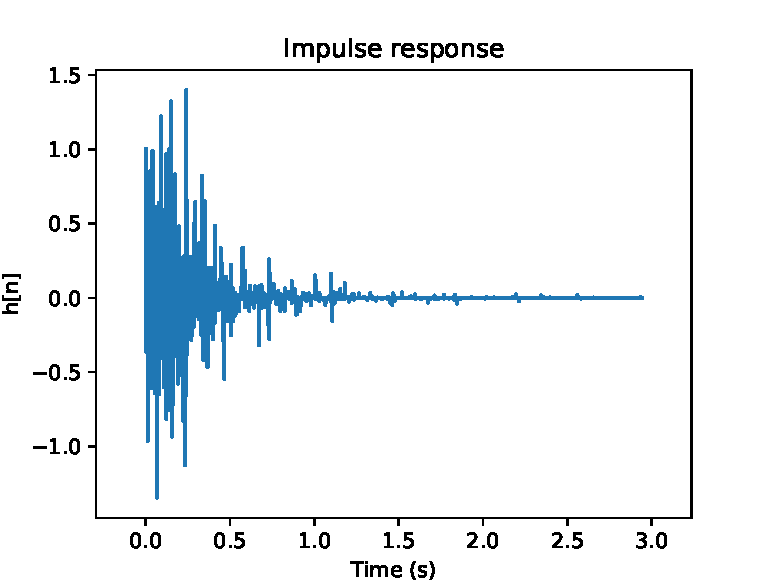
\includegraphics[width=\textwidth]{Applications/figures/reverb.pdf}
\end{center}
\caption{An impulse response that models the acoustics of a large space, with echoes at up to 3 seconds time delay.}
\label{fig:room_model}
\end{marginfigure}


One way to characterize $h[n]$ for a room is to simply measure it. One
emits a very short discrete unit impulse $\delta[n]$ using a high
quality speaker, and then measures the echoes for this pulse to
obtain:
\begin{equation}
h[n] = \sum_{r=0}^M h[r]\delta[n-r]\,\,.
\end{equation}
Another possibility is to model the impulse response $h[n]$ by making
assumptions about the delays of the reflecting surfaces in a room or
space.

The following snippet of code demonstrates modeling of the acoustics
of a room using a modeled impulse response for a room.

\lstinputlisting[language=Python,caption={\texttt{018\_reverb/reverb.py}},label=lst:exercise_reverb]{code/018_reverb/reverb.py}